\documentclass[11pt,a4paper]{article}

\usepackage[T1]{fontenc}
\usepackage[utf8]{inputenc}
\usepackage{lmodern}
\usepackage[margin=2.2cm]{geometry}
\usepackage{amsmath,amssymb,amsthm,mathtools}
\usepackage{bm}
\usepackage{booktabs}
\usepackage{array}
\usepackage{xcolor}
\usepackage{tikz}
\usetikzlibrary{arrows.meta,calc,positioning}
\usepackage{enumitem}
\usepackage[colorlinks=true,linkcolor=blue!60!black,citecolor=blue!60!black,urlcolor=blue!60!black]{hyperref}

\setlength{\emergencystretch}{3em}
\setlength{\parskip}{4pt}

\definecolor{atomblue}{RGB}{41,128,185}
\definecolor{defectred}{RGB}{211,47,47}
\definecolor{okgreen}{RGB}{46,125,50}
\definecolor{boxbg}{RGB}{245,248,252}
\definecolor{boxframe}{RGB}{180,200,225}

\newcommand{\R}{\mathbb{R}}
\newcommand{\Z}{\mathbb{Z}}
\newcommand{\T}{^{\mathsf T}}
\newcommand{\code}[1]{\texttt{#1}}

\newenvironment{keyidea}[1][Key Physical Idea]{%
  \par\medskip\noindent
  \begin{tikzpicture}
    \node[draw=boxframe,fill=boxbg,rounded corners=4pt,inner sep=10pt,text width=\dimexpr\textwidth-22pt\relax] (box) \bgroup
    \textbf{\textcolor{blue!60!black}{#1.}}\par\smallskip
}{%
    \egroup;
  \end{tikzpicture}\par\medskip
}

\title{\textbf{Computing the Aligned Deformation Gradient $\mathbf{F}_{\text{aligned}}$}\\[6pt]
\large Removing Arbitrary Mesh-Triangulation Orientations in First Piola--Kirchhoff and Projected Stress Post-Processing}
\author{MTM Lattice-Triangulation Documentation}
\date{October 2026}

\begin{document}
\maketitle

\begin{abstract}
\noindent
In a 2D triangulated crystal mesh, each triangular element's raw deformation gradient $\mathbf{F}$ is defined relative to a single fixed canonical right-angled reference triangle. Because a unit cell consists of both lower-left ($\triangle$) and upper-right ($\triangledown$) triangles, and because CGAL Delaunay triangulation assigns counterclockwise vertex indices $(v_0, v_1, v_2)$ starting from an arbitrary corner, the raw deformation gradient $\mathbf{F}$ contains an arbitrary discrete reference-space transformation $\mathbf{N}^{-1} \in SL(2,\Z)$ on the right. While the metric tensor $\mathbf{C} = \mathbf{F}\T\mathbf{F}$ (after Lagrange reduction), the strain energy $W(\mathbf{C}_{\text{red}})$, and the Cauchy stress $\boldsymbol{\sigma}$ are strictly invariant under $\mathbf{N} \in SL(2,\Z)$, the First Piola--Kirchhoff stress $\mathbf{P} = \partial W / \partial \mathbf{F}$ and the Projected Stress $\tau = \mathbf{m}\cdot(\mathbf{P}\mathbf{n})$ Carry an explicit reference-space index and therefore flip sign or swap columns between neighboring triangles. This document explains how $\mathbf{F}_{\text{aligned}} = \mathbf{F}\mathbf{N}$ is computed and how the entire post-processing stress pipeline follows directly from $\mathbf{F}_{\text{aligned}}$ without altering any downstream formulas.
\end{abstract}

\tableofcontents

% ============================================================================
\section{Why the Raw Deformation Gradient $\mathbf{F}$ Depends on Triangle Labelling}
% ============================================================================

Let a triangular element have current deformed vertex positions $\mathbf{x}_0, \mathbf{x}_1, \mathbf{x}_2 \in \R^2$ ordered counterclockwise ($\det[\mathbf{x}_1-\mathbf{x}_0,\;\mathbf{x}_2-\mathbf{x}_0] > 0$). In the MTM code (\code{ElementTriangle2D::calculate\_deformation\_gradient}), every element is mapped from the \textbf{same canonical right-angled reference triangle} with edge matrix
\begin{equation}
  \mathbf{X}_{\text{ref}} =
  \begin{pmatrix}
    a_0 & 0 \\
    0 & a_0
  \end{pmatrix},
  \qquad
  \mathbf{X}_{\text{ref}}^{-1} = \frac{1}{a_0}
  \begin{pmatrix}
    1 & 0 \\
    0 & 1
  \end{pmatrix}.
\end{equation}
Denoting the two deformed edge vectors emanating from vertex $v_0$ by
\begin{equation}
  \mathbf{e}_1 = \mathbf{x}_1 - \mathbf{x}_0, \qquad
  \mathbf{e}_2 = \mathbf{x}_2 - \mathbf{x}_0, \qquad
  \mathbf{E} = \begin{bmatrix} \mathbf{e}_1 & \mathbf{e}_2 \end{bmatrix} \in \R^{2\times 2},
\end{equation}
the raw element deformation gradient is computed as
\begin{equation}
  \mathbf{F} = \frac{1}{a_0}\,\mathbf{E}\,\mathbf{X}_{\text{ref}}^{-1}
  \qquad\text{(equal to $\mathbf{E}$ when normalized by $a_0=1$).}
  \label{eq:raw_F}
\end{equation}

Two purely geometric ambiguities enter Eq.~\eqref{eq:raw_F} before any physical elastic deformation occurs:

\subsection{Ambiguity 1: The 4 Discrete $90^\circ$ Half-Cell Orientations ($\mathbf{R}_0, \mathbf{R}_1, \mathbf{R}_2, \mathbf{R}_3$)}
In a finite-element mesh with dynamic Delaunay remeshing, triangles are destroyed and re-created during plastic avalanches, so individual triangles do not store their own initial node coordinates. Instead, every triangle in the mesh is compared against the \textbf{single bottom-left template triangle} $p_1=(0,0),\; p_2=(a_0,0),\; p_3=(0,a_0)$ via the fixed shape-derivative matrix $\texttt{dndx}$.

However, a unit square $[0,1]\times[0,1]$ has four corners and can be split along either diagonal ($\backslash$ or $/$) into four possible right-angled half-cell triangles whose $90^\circ$ corner sits at $(0,0)$, $(1,0)$, $(1,1)$, or $(0,1)$. Even when the origin $v_0$ is placed directly at the $90^\circ$ corner of each triangle, walking counterclockwise produces four different raw deformation gradients rotated by $0^\circ, 90^\circ, 180^\circ, 270^\circ$:
\begin{enumerate}[noitemsep]
  \item \textbf{Bottom-left triangle} ($90^\circ$ corner at $v_0=(0,0) \to (1,0) \to (0,1)$, rotation $0^\circ$):
  \begin{equation}
    \mathbf{e}_1 = \begin{pmatrix} 1 \\ 0 \end{pmatrix}, \quad
    \mathbf{e}_2 = \begin{pmatrix} 0 \\ 1 \end{pmatrix}
    \quad\Longrightarrow\quad
    \mathbf{F} = \begin{pmatrix} 1 & 0 \\ 0 & 1 \end{pmatrix} = \mathbf{R}_0.
  \end{equation}
  \item \textbf{Bottom-right triangle} ($90^\circ$ corner at $v_0=(1,0) \to (1,1) \to (0,0)$, rotation $90^\circ$):
  \begin{equation}
    \mathbf{e}_1 = \begin{pmatrix} 0 \\ 1 \end{pmatrix}, \quad
    \mathbf{e}_2 = \begin{pmatrix} -1 \\ 0 \end{pmatrix}
    \quad\Longrightarrow\quad
    \mathbf{F} = \begin{pmatrix} 0 & -1 \\ 1 & 0 \end{pmatrix} = \mathbf{R}_1.
  \end{equation}
  \item \textbf{Top-right triangle} ($90^\circ$ corner at $v_0=(1,1) \to (0,1) \to (1,0)$, rotation $180^\circ$):
  \begin{equation}
    \mathbf{e}_1 = \begin{pmatrix} -1 \\ 0 \end{pmatrix}, \quad
    \mathbf{e}_2 = \begin{pmatrix} 0 \\ -1 \end{pmatrix}
    \quad\Longrightarrow\quad
    \mathbf{F} = \begin{pmatrix} -1 & 0 \\ 0 & -1 \end{pmatrix} = \mathbf{R}_2.
  \end{equation}
  \item \textbf{Top-left triangle} ($90^\circ$ corner at $v_0=(0,1) \to (0,0) \to (1,1)$, rotation $270^\circ$):
  \begin{equation}
    \mathbf{e}_1 = \begin{pmatrix} 0 \\ -1 \end{pmatrix}, \quad
    \mathbf{e}_2 = \begin{pmatrix} 1 \\ 0 \end{pmatrix}
    \quad\Longrightarrow\quad
    \mathbf{F} = \begin{pmatrix} 0 & 1 \\ -1 & 0 \end{pmatrix} = \mathbf{R}_3.
  \end{equation}
\end{enumerate}
Right-multiplying $\mathbf{F}$ by $\mathbf{R}_r\T$ ($r \in \{0,1,2,3\}$) rotates the local reference axes of the triangle by $-0^\circ, -90^\circ, -180^\circ, -270^\circ$, bringing all four half-square triangles back to $\mathbf{F}\mathbf{R}_r\T = +\mathbf{I}$.

\begin{figure}[htbp]
\centering
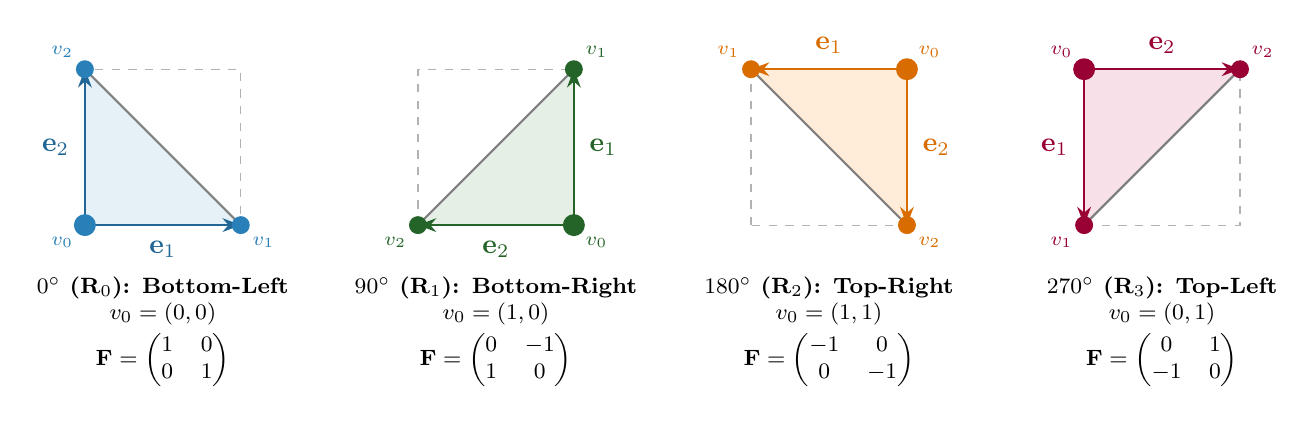
\begin{tikzpicture}[scale=1.8, >=Stealth]
  % R0: 0 deg (bottom-left)
  \begin{scope}[xshift=0cm]
    \draw[dashed, gray!60] (0,0) rectangle (1.1,1.1);
    \fill[atomblue!12] (0,0) -- (1.1,0) -- (0,1.1) -- cycle;
    \draw[thick, gray] (1.1,0) -- (0,1.1);
    \draw[thick, atomblue!80!black, ->] (0,0) -- (1.1,0) node[midway, below=2pt] {$\mathbf{e}_1$};
    \draw[thick, atomblue!80!black, ->] (0,0) -- (0,1.1) node[midway, left=2pt] {$\mathbf{e}_2$};
    \fill[atomblue] (0,0) circle (2.2pt) node[below left=1pt, font=\scriptsize] {$v_0$};
    \fill[atomblue] (1.1,0) circle (1.8pt) node[below right=1pt, font=\scriptsize] {$v_1$};
    \fill[atomblue] (0,1.1) circle (1.8pt) node[above left=1pt, font=\scriptsize] {$v_2$};
    \node[align=center, font=\footnotesize] at (0.55,-0.75) {\textbf{$0^\circ$ ($\mathbf{R}_0$): Bottom-Left}\\$v_0=(0,0)$\\[2pt]$\mathbf{F} = \begin{pmatrix} 1 & 0 \\ 0 & 1 \end{pmatrix}$};
  \end{scope}

  % R1: 90 deg (bottom-right)
  \begin{scope}[xshift=2.35cm]
    \draw[dashed, gray!60] (0,0) rectangle (1.1,1.1);
    \fill[okgreen!12] (1.1,0) -- (1.1,1.1) -- (0,0) -- cycle;
    \draw[thick, gray] (1.1,1.1) -- (0,0);
    \draw[thick, okgreen!80!black, ->] (1.1,0) -- (1.1,1.1) node[midway, right=2pt] {$\mathbf{e}_1$};
    \draw[thick, okgreen!80!black, ->] (1.1,0) -- (0,0) node[midway, below=2pt] {$\mathbf{e}_2$};
    \fill[okgreen!80!black] (1.1,0) circle (2.2pt) node[below right=1pt, font=\scriptsize] {$v_0$};
    \fill[okgreen!80!black] (1.1,1.1) circle (1.8pt) node[above right=1pt, font=\scriptsize] {$v_1$};
    \fill[okgreen!80!black] (0,0) circle (1.8pt) node[below left=1pt, font=\scriptsize] {$v_2$};
    \node[align=center, font=\footnotesize] at (0.55,-0.75) {\textbf{$90^\circ$ ($\mathbf{R}_1$): Bottom-Right}\\$v_0=(1,0)$\\[2pt]$\mathbf{F} = \begin{pmatrix} 0 & -1 \\ 1 & 0 \end{pmatrix}$};
  \end{scope}

  % R2: 180 deg (top-right)
  \begin{scope}[xshift=4.7cm]
    \draw[dashed, gray!60] (0,0) rectangle (1.1,1.1);
    \fill[orange!15] (1.1,1.1) -- (0,1.1) -- (1.1,0) -- cycle;
    \draw[thick, gray] (0,1.1) -- (1.1,0);
    \draw[thick, orange!85!black, ->] (1.1,1.1) -- (0,1.1) node[midway, above=2pt] {$\mathbf{e}_1$};
    \draw[thick, orange!85!black, ->] (1.1,1.1) -- (1.1,0) node[midway, right=2pt] {$\mathbf{e}_2$};
    \fill[orange!85!black] (1.1,1.1) circle (2.2pt) node[above right=1pt, font=\scriptsize] {$v_0$};
    \fill[orange!85!black] (0,1.1) circle (1.8pt) node[above left=1pt, font=\scriptsize] {$v_1$};
    \fill[orange!85!black] (1.1,0) circle (1.8pt) node[below right=1pt, font=\scriptsize] {$v_2$};
    \node[align=center, font=\footnotesize] at (0.55,-0.75) {\textbf{$180^\circ$ ($\mathbf{R}_2$): Top-Right}\\$v_0=(1,1)$\\[2pt]$\mathbf{F} = \begin{pmatrix} -1 & 0 \\ 0 & -1 \end{pmatrix}$};
  \end{scope}

  % R3: 270 deg (top-left)
  \begin{scope}[xshift=7.05cm]
    \draw[dashed, gray!60] (0,0) rectangle (1.1,1.1);
    \fill[purple!12] (0,1.1) -- (0,0) -- (1.1,1.1) -- cycle;
    \draw[thick, gray] (0,0) -- (1.1,1.1);
    \draw[thick, purple!80!black, ->] (0,1.1) -- (0,0) node[midway, left=2pt] {$\mathbf{e}_1$};
    \draw[thick, purple!80!black, ->] (0,1.1) -- (1.1,1.1) node[midway, above=2pt] {$\mathbf{e}_2$};
    \fill[purple!80!black] (0,1.1) circle (2.2pt) node[above left=1pt, font=\scriptsize] {$v_0$};
    \fill[purple!80!black] (0,0) circle (1.8pt) node[below left=1pt, font=\scriptsize] {$v_1$};
    \fill[purple!80!black] (1.1,1.1) circle (1.8pt) node[above right=1pt, font=\scriptsize] {$v_2$};
    \node[align=center, font=\footnotesize] at (0.55,-0.75) {\textbf{$270^\circ$ ($\mathbf{R}_3$): Top-Left}\\$v_0=(0,1)$\\[2pt]$\mathbf{F} = \begin{pmatrix} 0 & 1 \\ -1 & 0 \end{pmatrix}$};
  \end{scope}
\end{tikzpicture}
\caption{\textbf{What the 4 discrete rotations $\mathbf{R}_r$ do:} A unit square $[0,1]\times[0,1]$ (dashed outline) can contain four different right-angled triangle orientations depending on which half of the square the triangle occupies and which diagonal ($\backslash$ or $/$) splits the cell. Right-multiplying by $\mathbf{R}_r\T$ rotates all four orientations back to $+\mathbf{I}$.}
\label{fig:four_rotations}
\end{figure}

\subsection{Ambiguity 2: The 3 Cyclic Counterclockwise Vertex Shifts in CGAL ($\mathbf{M}_0, \mathbf{M}_1, \mathbf{M}_2$)}
Now consider a \textbf{single fixed triangle} in space---for example, the bottom-left triangle with corners at $(0,0)$, $(1,0)$, and $(0,1)$. When CGAL builds or remeshes the Delaunay triangulation, any of the triangle's three corners may be listed first as $v_0$, provided $(v_0, v_1, v_2)$ remains counterclockwise. Cycling which corner is chosen as the origin $v_0$ transforms the edge matrix $\mathbf{E} = [\mathbf{e}_1, \mathbf{e}_2]$ by right-multiplication with a unimodular matrix $\mathbf{M}_p \in SL(2,\Z)$:
\begin{enumerate}[noitemsep]
  \item \textbf{No shift ($\mathbf{M}_0$)}, origin at $v_0=(0,0) \to v_1=(1,0) \to v_2=(0,1)$:
  \begin{equation}
    [\mathbf{e}_1,\; \mathbf{e}_2]
    = [\mathbf{e}_1,\; \mathbf{e}_2]
    \underbrace{\begin{pmatrix} 1 & 0 \\ 0 & 1 \end{pmatrix}}_{\mathbf{M}_0}.
  \end{equation}
  \item \textbf{One cyclic shift ($\mathbf{M}_1$)}, origin shifted to $v_0'=(1,0) \to v_1'=(0,1) \to v_2'=(0,0)$:
  new edges are $\mathbf{e}_1' = \mathbf{x}_2 - \mathbf{x}_1 = -\mathbf{e}_1 + \mathbf{e}_2$ and $\mathbf{e}_2' = \mathbf{x}_0 - \mathbf{x}_1 = -\mathbf{e}_1$:
  \begin{equation}
    [\mathbf{e}_1',\; \mathbf{e}_2']
    = [\mathbf{e}_1,\; \mathbf{e}_2]
    \underbrace{\begin{pmatrix} -1 & -1 \\ 1 & 0 \end{pmatrix}}_{\mathbf{M}_1}.
  \end{equation}
  \item \textbf{Two cyclic shifts ($\mathbf{M}_2$)}, origin shifted to $v_0''=(0,1) \to v_1''=(0,0) \to v_2''=(1,0)$:
  new edges are $\mathbf{e}_1'' = \mathbf{x}_0 - \mathbf{x}_2 = -\mathbf{e}_2$ and $\mathbf{e}_2'' = \mathbf{x}_1 - \mathbf{x}_2 = \mathbf{e}_1 - \mathbf{e}_2$:
  \begin{equation}
    [\mathbf{e}_1'',\; \mathbf{e}_2'']
    = [\mathbf{e}_1,\; \mathbf{e}_2]
    \underbrace{\begin{pmatrix} 0 & 1 \\ -1 & -1 \end{pmatrix}}_{\mathbf{M}_2}.
  \end{equation}
\end{enumerate}
Note that $\det\mathbf{M}_0 = \det\mathbf{M}_1 = \det\mathbf{M}_2 = +1$, and $\mathbf{M}_0, \mathbf{M}_1, \mathbf{M}_2 \in SL(2,\Z)$ form a cyclic group of order $3$ ($\mathbf{M}_1^2 = \mathbf{M}_2$, $\mathbf{M}_1^3 = \mathbf{I}$, so $\mathbf{M}_1^{-1} = \mathbf{M}_2$ and $\mathbf{M}_2^{-1} = \mathbf{M}_1$).

\begin{figure}[htbp]
\centering
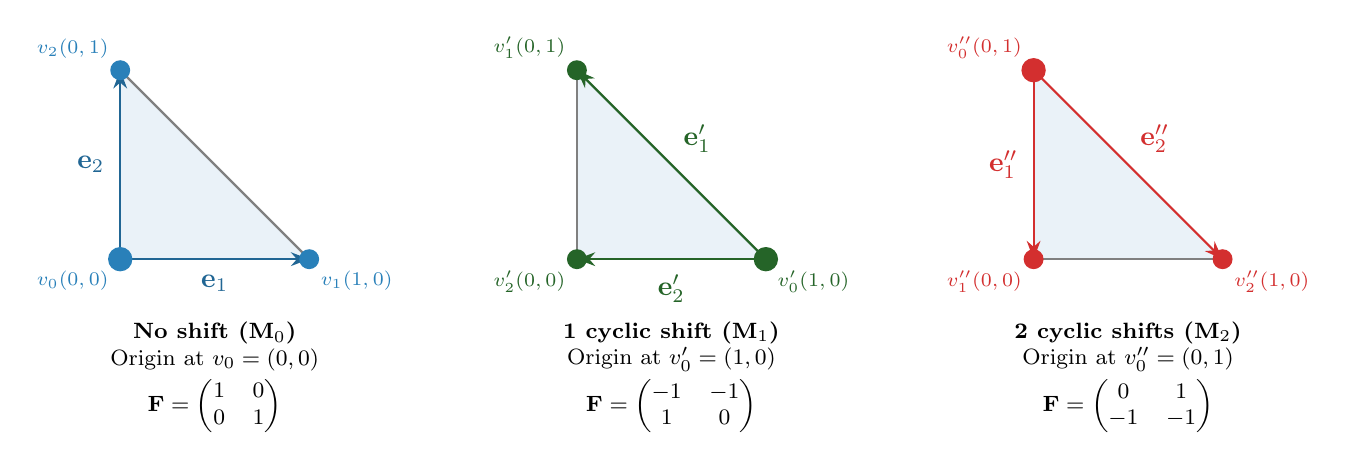
\begin{tikzpicture}[scale=2.0, >=Stealth]
  % Left: M0 (no shift, origin at (0,0))
  \begin{scope}[xshift=0cm]
    \fill[atomblue!10] (0,0) -- (1.2,0) -- (0,1.2) -- cycle;
    \draw[thick, gray] (1.2,0) -- (0,1.2);
    \draw[thick, atomblue!80!black, ->] (0,0) -- (1.2,0) node[midway, below=2pt] {$\mathbf{e}_1$};
    \draw[thick, atomblue!80!black, ->] (0,0) -- (0,1.2) node[midway, left=2pt] {$\mathbf{e}_2$};
    \fill[atomblue] (0,0) circle (2.2pt) node[below left=1pt, font=\scriptsize] {$v_0(0,0)$};
    \fill[atomblue] (1.2,0) circle (1.8pt) node[below right=1pt, font=\scriptsize] {$v_1(1,0)$};
    \fill[atomblue] (0,1.2) circle (1.8pt) node[above left=1pt, font=\scriptsize] {$v_2(0,1)$};
    \node[align=center, font=\footnotesize] at (0.6,-0.75) {\textbf{No shift ($\mathbf{M}_0$)}\\Origin at $v_0=(0,0)$\\[2pt]$\mathbf{F} = \begin{pmatrix} 1 & 0 \\ 0 & 1 \end{pmatrix}$};
  \end{scope}

  % Middle: M1 (1 cyclic shift, origin at (1,0))
  \begin{scope}[xshift=2.9cm]
    \fill[atomblue!10] (0,0) -- (1.2,0) -- (0,1.2) -- cycle;
    \draw[thick, gray] (0,0) -- (0,1.2);
    \draw[thick, okgreen!80!black, ->] (1.2,0) -- (0,1.2) node[midway, above right=1pt] {$\mathbf{e}_1'$};
    \draw[thick, okgreen!80!black, ->] (1.2,0) -- (0,0) node[midway, below=2pt] {$\mathbf{e}_2'$};
    \fill[okgreen!80!black] (1.2,0) circle (2.2pt) node[below right=1pt, font=\scriptsize] {$v_0'(1,0)$};
    \fill[okgreen!80!black] (0,1.2) circle (1.8pt) node[above left=1pt, font=\scriptsize] {$v_1'(0,1)$};
    \fill[okgreen!80!black] (0,0) circle (1.8pt) node[below left=1pt, font=\scriptsize] {$v_2'(0,0)$};
    \node[align=center, font=\footnotesize] at (0.6,-0.75) {\textbf{1 cyclic shift ($\mathbf{M}_1$)}\\Origin at $v_0'=(1,0)$\\[2pt]$\mathbf{F} = \begin{pmatrix} -1 & -1 \\ 1 & 0 \end{pmatrix}$};
  \end{scope}

  % Right: M2 (2 cyclic shifts, origin at (0,1))
  \begin{scope}[xshift=5.8cm]
    \fill[atomblue!10] (0,0) -- (1.2,0) -- (0,1.2) -- cycle;
    \draw[thick, gray] (0,0) -- (1.2,0);
    \draw[thick, defectred, ->] (0,1.2) -- (0,0) node[midway, left=2pt] {$\mathbf{e}_1''$};
    \draw[thick, defectred, ->] (0,1.2) -- (1.2,0) node[midway, above right=1pt] {$\mathbf{e}_2''$};
    \fill[defectred] (0,1.2) circle (2.2pt) node[above left=1pt, font=\scriptsize] {$v_0''(0,1)$};
    \fill[defectred] (0,0) circle (1.8pt) node[below left=1pt, font=\scriptsize] {$v_1''(0,0)$};
    \fill[defectred] (1.2,0) circle (1.8pt) node[below right=1pt, font=\scriptsize] {$v_2''(1,0)$};
    \node[align=center, font=\footnotesize] at (0.6,-0.75) {\textbf{2 cyclic shifts ($\mathbf{M}_2$)}\\Origin at $v_0''=(0,1)$\\[2pt]$\mathbf{F} = \begin{pmatrix} 0 & 1 \\ -1 & -1 \end{pmatrix}$};
  \end{scope}
\end{tikzpicture}
\caption{\textbf{What the 3 cyclic shifts $\mathbf{M}_p$ do:} All three panels show the \textbf{exact same physical triangle} with vertices at $(0,0)$, $(1,0)$, and $(0,1)$. Depending on which of the 3 corners CGAL lists first as $v_0$, the two edge vectors emanating from that corner change according to $\mathbf{M}_0$, $\mathbf{M}_1$, or $\mathbf{M}_2$. Multiplying on the right by $\mathbf{M}_p$ shifts the local origin $v_0$ back to the $90^\circ$ corner $(0,0)$.}
\label{fig:tri_orientations}
\end{figure}

% ============================================================================
\section{Single Unified Formula for Computing $\mathbf{F}_{\text{aligned}}$}
% ============================================================================

Because a crystal in the Zanzotto potential can contain both square and triangular (hexagonal) phases simultaneously (as well as heavily sheared dislocation cores), we use a \textbf{single unified formula} for every element without branching on lattice type.

In the Lagrange fundamental domain $0 \le 2\,C_{12} \le C_{11} \le C_{22}$:
\begin{itemize}[noitemsep]
  \item The \textbf{square phase} sits at the left boundary $F_{12} = 0$: $\mathbf{F}_{\text{sq}} = \begin{pmatrix} 1 & 0 \\ 0 & 1 \end{pmatrix}$.
  \item The \textbf{triangular (hexagonal) phase} sits at the right boundary $F_{12} = +\tfrac{1}{2}a_0$: $\mathbf{F}_{\text{tri}} = a_0\begin{pmatrix} 1 & +1/2 \\ 0 & \sqrt{3}/2 \end{pmatrix}$.
\end{itemize}
By placing the target reference matrix $\mathbf{F}_{\text{target}}$ at the \textbf{midpoint} ($F_{12} = 1/4$) of the fundamental domain between the square and triangular wells,
\begin{equation}
  \mathbf{F}_{\text{target}} = \mathbf{R}(\theta_0)
  \begin{pmatrix}
    1 & 1/4 \\
    0 & 1
  \end{pmatrix},
  \qquad
  \mathbf{R}(\theta_0) =
  \begin{pmatrix}
    \cos\theta_0 & -\sin\theta_0 \\
    \sin\theta_0 & \cos\theta_0
  \end{pmatrix},
\end{equation}
both the square phase ($F_{12}=0$) and the triangular phase ($F_{12}=+1/2$) are at distance $\approx 1/4$ from $\mathbf{F}_{\text{target}}$, while the reflected obtuse triangular orientation ($F_{12}=-1/2$) and unaligned square orientations ($F_{12}=\pm 1$) are at distance $\ge 3/4$.

Combining the $3$ cyclic triangle vertex permutations $\mathbf{M}_p$ ($p \in \{0,1,2\}$) with the $4$ discrete $90^\circ$ reference rotations $\mathbf{R}_r \in SL(2,\Z)$,
\begin{equation}
  \mathbf{R}_0 = \begin{pmatrix} 1 & 0 \\ 0 & 1 \end{pmatrix}, \quad
  \mathbf{R}_1 = \begin{pmatrix} 0 & -1 \\ 1 & 0 \end{pmatrix}, \quad
  \mathbf{R}_2 = \begin{pmatrix} -1 & 0 \\ 0 & -1 \end{pmatrix}, \quad
  \mathbf{R}_3 = \begin{pmatrix} 0 & 1 \\ -1 & 0 \end{pmatrix},
\end{equation}
yields the single formula used for all elements:
\begin{equation}
  \boxed{
  \mathbf{F}_{\text{aligned}} = \operatorname*{arg\,min}_{\substack{p \in \{0,1,2\} \\ r \in \{0,1,2,3\}}}
  \left\| \mathbf{F}\,\mathbf{M}_p\,\mathbf{R}_r\T - \mathbf{F}_{\text{target}} \right\|_F^2
  }
  \label{eq:f_aligned_sq}
\end{equation}
where $\|\mathbf{A}\|_F^2 = \operatorname{tr}(\mathbf{A}\T\mathbf{A}) = \sum_{i,j} A_{ij}^2$ is the squared Frobenius norm (\code{.squaredNorm()} in Eigen).

% ============================================================================
\section{Why Nothing Downstream Needs to Change Once $\mathbf{F}_{\text{aligned}}$ is Found}
% ============================================================================

\begin{keyidea}[Drop-In Replacement Property]
Because $\mathbf{F}_{\text{aligned}} = \mathbf{F}\mathbf{N}$ with $\mathbf{N} \in SL(2,\Z)$ ($\det\mathbf{N} = +1$), $\mathbf{F}_{\text{aligned}}$ belongs to the \textbf{exact same $GL(2,\Z)$ lattice equivalence class} as $\mathbf{F}$. Therefore, replacing $\mathbf{F}$ by $\mathbf{F}_{\text{aligned}}$ at the very start of the stress routine leaves the reduced metric $\mathbf{C}_{\text{red}}$, the strain energy $W$, and the Cauchy stress $\boldsymbol{\sigma}$ mathematically unchanged, while automatically aligning the First Piola--Kirchhoff stress $\mathbf{P}_{\text{aligned}}$ and Projected Stress $\tau_{\text{aligned}}$.
\end{keyidea}

Once $\mathbf{F}_{\text{aligned}}$ is computed via Eq.~\eqref{eq:f_aligned_sq}, the existing stress pipeline proceeds verbatim:

\begin{enumerate}
  \item \textbf{Aligned Right Cauchy--Green Metric Tensor}:
  \begin{equation}
    \mathbf{C}_{\text{aligned}} = \mathbf{F}_{\text{aligned}}\T \mathbf{F}_{\text{aligned}}
    = \mathbf{N}\T \mathbf{F}\T \mathbf{F} \mathbf{N}
    = \mathbf{N}\T \mathbf{C} \mathbf{N}.
  \end{equation}

  \item \textbf{Lagrange Reduction to the Fundamental Domain}:
  Applying \code{lagrange::reduce}$(\mathbf{C}_{\text{aligned}})$ finds the unimodular reduction matrix $\mathbf{M} \in GL(2,\Z)$ that maps $\mathbf{C}_{\text{aligned}}$ into the unique Lagrange-reduced metric $\mathbf{C}_{\text{red}}$:
  \begin{equation}
    \mathbf{C}_{\text{red}} = \mathbf{M}\T \mathbf{C}_{\text{aligned}} \mathbf{M}.
  \end{equation}
  For bulk elastic elements, $\mathbf{C}_{\text{aligned}}$ is already in the fundamental domain, so $\mathbf{M} = \mathbf{I}$. For plastically slipped elements (or elements at dislocation cores), $\mathbf{M}$ automatically strips the plastic lattice shear!

  \item \textbf{Constitutive Energy Derivative}:
  \begin{equation}
    \mathbf{S}_{\text{red}} = \frac{1}{A_{\text{cell}}} \frac{\partial W(\mathbf{C}_{\text{red}})}{\partial \mathbf{C}_{\text{red}}}.
  \end{equation}

  \item \textbf{Aligned First Piola--Kirchhoff Stress Tensor}:
  \begin{equation}
    \boxed{
    \mathbf{P}_{\text{aligned}} = 2\,\mathbf{F}_{\text{aligned}}\,\mathbf{M}\,\mathbf{S}_{\text{red}}\,\mathbf{M}\T.
    }
    \label{eq:P_aligned}
  \end{equation}

  \item \textbf{Cauchy Stress Tensor (Identical to Unaligned $\boldsymbol{\sigma}$)}:
  \begin{equation}
    \boxed{
    \boldsymbol{\sigma}_{\text{aligned}}
    = \frac{1}{\det\mathbf{F}_{\text{aligned}}} \mathbf{P}_{\text{aligned}} \mathbf{F}_{\text{aligned}}\T
    = \frac{2}{\det\mathbf{F}_{\text{aligned}}}
      (\mathbf{F}_{\text{aligned}}\mathbf{M})\,\mathbf{S}_{\text{red}}\,(\mathbf{F}_{\text{aligned}}\mathbf{M})\T
    = \boldsymbol{\sigma}.
    }
    \label{eq:cauchy_aligned}
  \end{equation}
  \emph{Proof of invariance:} Since $\mathbf{C}_{\text{aligned}} = \mathbf{N}\T \mathbf{C} \mathbf{N}$ and $\det\mathbf{N} = 1$, both $\mathbf{C}$ and $\mathbf{C}_{\text{aligned}}$ reduce to the same canonical metric $\mathbf{C}_{\text{red}}$ in the fundamental domain, with $\mathbf{F}_{\text{aligned}}\mathbf{M} = \mathbf{F}\mathbf{M}_{\text{orig}}$ (up to lattice point-group symmetries of $W$). Hence $(\mathbf{F}_{\text{aligned}}\mathbf{M})\mathbf{S}_{\text{red}}(\mathbf{F}_{\text{aligned}}\mathbf{M})\T$ and $\det\mathbf{F}_{\text{aligned}} = \det\mathbf{F}\det\mathbf{N} = \det\mathbf{F}$ are completely invariant.

  \item \textbf{Lab-Frame First Piola--Kirchhoff and Projected Stress}:
  When the crystal is rotated by $\theta_0$ (rotate-and-cut CSL or fixed-BC supercell) and sheared in the lab frame with $\mathbf{F}_{\text{ext}}(\alpha) = \begin{pmatrix} 1 & \alpha \\ 0 & 1 \end{pmatrix}$, rotating the reference index of $\mathbf{P}_{\text{aligned}}$ by $\mathbf{R}(\theta_0)\T$ gives the lab-frame First Piola--Kirchhoff tensor and the work-conjugate projected stress:
  \begin{equation}
    \mathbf{P}_{\text{lab}} = \mathbf{P}_{\text{aligned}}\,\mathbf{R}(\theta_0)\T, \qquad
    \boxed{
    \sigma_{\text{proj}} = \mathbf{P}_{\text{lab}} : \frac{\partial \mathbf{F}_{\text{ext}}}{\partial \alpha}
    = (\mathbf{P}_{\text{lab}})_{12}
    = P_{11}^{\text{aligned}}\sin\theta_0 + P_{12}^{\text{aligned}}\cos\theta_0.
    }
  \end{equation}
\end{enumerate}

% ============================================================================
\section{Worked Numerical Examples from Simulation}
% ============================================================================

The tables below show actual element tensors extracted from a $100 \times 100$ square-lattice simulation (\code{checkpoint\_00007.chk} at external stretch $\alpha = 0.1419$).

\subsection{Example 1: Alternating Bulk Elements (\code{Element 0} vs.\ \code{Element 1})}
\code{Element 0} is a lower-left triangle ($\triangle$) whose CGAL vertex order shifted its columns by $\mathbf{M}_2$, while \code{Element 1} is the adjacent upper-right triangle ($\triangledown$) with opposite orientation:

\begin{center}
\renewcommand{\arraystretch}{1.35}
\small
\begin{tabular}{@{}lll@{}}
\toprule
\textbf{Quantity} & \textbf{Element 0 (Bulk $\triangle$)} & \textbf{Element 1 (Bulk $\triangledown$)} \\
\midrule
Raw $\mathbf{F}$ &
$\begin{pmatrix} -1.15035 & -0.00011 \\ 0.00010 & 0.86927 \end{pmatrix}$ &
$\begin{pmatrix} -1.15039 & 1.15024 \\ 0.00007 & -0.86937 \end{pmatrix}$ \\[10pt]
Aligned $\mathbf{F}_{\text{aligned}}$ &
$\begin{pmatrix} 1.15024 & -0.00011 \\ -0.00010 & 0.86927 \end{pmatrix}$ &
$\begin{pmatrix} 1.15024 & -0.00015 \\ -0.00007 & 0.86930 \end{pmatrix}$ \\[10pt]
Raw $\mathbf{P}$ &
$\begin{pmatrix} +0.39109 & -0.00013 \\ +0.00037 & -0.50618 \end{pmatrix}$ &
$\begin{pmatrix} +0.39137 & -0.00004 \\ -0.00009 & \mathbf{+0.50583} \end{pmatrix}$ \\[10pt]
Aligned $\mathbf{P}_{\text{aligned}}$ &
$\begin{pmatrix} -0.39109 & -0.00013 \\ -0.00037 & \mathbf{-0.50618} \end{pmatrix}$ &
$\begin{pmatrix} -0.39137 & +0.00004 \\ +0.00009 & \mathbf{-0.50583} \end{pmatrix}$ \\[10pt]
Raw Cauchy $\boldsymbol{\sigma}$ &
$\begin{pmatrix} -0.44985 & -0.00036 \\ -0.00036 & -0.44001 \end{pmatrix}$ &
$\begin{pmatrix} -0.45017 & +0.00010 \\ +0.00010 & -0.43972 \end{pmatrix}$ \\[10pt]
Aligned Cauchy $\boldsymbol{\sigma}_{\text{aligned}}$ &
$\begin{pmatrix} -0.44985 & -0.00036 \\ -0.00036 & -0.44001 \end{pmatrix}$ &
$\begin{pmatrix} -0.45017 & +0.00010 \\ +0.00010 & -0.43972 \end{pmatrix}$ \\
\bottomrule
\end{tabular}
\end{center}

Notice two key facts in this table:
\begin{itemize}[noitemsep]
  \item In the raw calculation, $P_{22}$ jumps from $-0.50618$ on \code{Element 0} to $+0.50583$ on \code{Element 1}, and $P_{11}$ has the wrong sign ($+0.391$) relative to $\sigma_{11}$ ($-0.450$).
  \item With $\mathbf{F}_{\text{aligned}}$, both elements have $\mathbf{F}_{\text{aligned}} \approx \operatorname{diag}(1.150, 0.869)$, $\mathbf{P}_{\text{aligned}} \approx \operatorname{diag}(-0.391, -0.506)$ with consistent sign across the entire mesh, and $\boldsymbol{\sigma}_{\text{aligned}} \equiv \boldsymbol{\sigma}$ to machine precision.
\end{itemize}

\subsection{Example 2: Plastically Slipped Elements (\code{Element 16328} and \code{Element 16126})}
For triangles that have undergone a plastic slip or sit next to a dislocation core, $\mathbf{F}_{\text{aligned}}$ removes the arbitrary CGAL vertex permutation while Lagrange reduction ($\mathbf{M}$ in Eq.~\eqref{eq:P_aligned}) reduces the slipped metric back to the fundamental elastic domain:

\begin{center}
\renewcommand{\arraystretch}{1.35}
\small
\begin{tabular}{@{}lll@{}}
\toprule
\textbf{Quantity} & \textbf{Element 16328 (Slipped)} & \textbf{Element 16126 (Slipped)} \\
\midrule
Raw $\mathbf{F}$ &
$\begin{pmatrix} -1.14893 & 2.29950 \\ -0.00297 & -0.87059 \end{pmatrix}$ &
$\begin{pmatrix} 1.15165 & 1.14974 \\ 0.87404 & -0.00331 \end{pmatrix}$ \\[10pt]
Aligned $\mathbf{F}_{\text{aligned}}$ &
$\begin{pmatrix} 1.15057 & -1.14893 \\ -0.87355 & -0.00297 \end{pmatrix}$ &
$\begin{pmatrix} 1.14974 & -1.15165 \\ -0.00331 & -0.87404 \end{pmatrix}$ \\[10pt]
Raw $\mathbf{P}$ &
$\begin{pmatrix} +0.38651 & -0.02527 \\ +0.02731 & +0.49104 \end{pmatrix}$ &
$\begin{pmatrix} -0.02266 & -0.37120 \\ -0.50378 & +0.02636 \end{pmatrix}$ \\[10pt]
Aligned $\mathbf{P}_{\text{aligned}}$ &
$\begin{pmatrix} -0.36124 & -0.38651 \\ +0.51835 & -0.02731 \end{pmatrix}$ &
$\begin{pmatrix} -0.37120 & +0.02266 \\ +0.02636 & +0.50378 \end{pmatrix}$ \\[10pt]
Raw Cauchy $\boldsymbol{\sigma}$ &
$\begin{pmatrix} -0.41502 & +0.03097 \\ +0.03097 & -0.45353 \end{pmatrix}$ &
$\begin{pmatrix} -0.42703 & -0.02985 \\ -0.02985 & -0.44042 \end{pmatrix}$ \\[10pt]
Aligned Cauchy $\boldsymbol{\sigma}_{\text{aligned}}$ &
$\begin{pmatrix} -0.41502 & +0.03097 \\ +0.03097 & -0.45353 \end{pmatrix}$ &
$\begin{pmatrix} -0.42703 & -0.02985 \\ -0.02985 & -0.44042 \end{pmatrix}$ \\
\bottomrule
\end{tabular}
\end{center}

\end{document}
